\documentclass{article}
\usepackage{tikz}
\usepackage{graphics}
\usepackage{pgfplots}
\begin{document}
\pagestyle{empty}


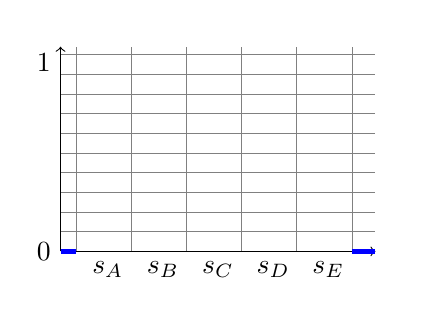
\begin{tikzpicture}
  \def\state{4.2}
  \def\statetwo{7.7}
  \def\xmin{4}
  \def\xmax{8}
  \def\ymin{0}
  \def\ymax{2.6}
  % grid
  \draw[style=help lines, ystep=0.25, xstep=0.7] (\xmin,\ymin) grid
  (\xmax,\ymax);
  % axes
  \draw[->] (\xmin,\ymin) -- (\xmax,\ymin) node[right] {};
  \node[right] at (\xmax,1) {};
  \node[above] (bli1) at (\xmin,\ymax) {}; %
  \draw[->] (\xmin,\ymin) -- (\xmin,\ymax) node {};

  % xticks and yticks
    \node at (4.6, \ymin) [below] {$s_A$};
    \node at (5.3, \ymin) [below] {$s_B$};
    \node at (6, \ymin) [below] {$s_C$};
    \node at (6.7, \ymin) [below] {$s_D$};
    \node at (7.4, \ymin) [below] {$s_E$};
    \node at (\xmin,\ymin) [left] {$0$};
    \node at (\xmin,2.4) [left] {$1$};

  % plot the data from the file data.dat
  \draw[color=red,ultra thick] plot[mark=*,mark size=1pt] file {data.dat};

   \draw[color=blue,ultra thick] (\xmin,0) -- (\state,0);
   \draw[color=blue,ultra thick] (\statetwo,0) -- (\xmax,0);
%   \draw[color=blue,ultra thick] (\state,0) -- (\state,2);
   \node[color=blue,ultra thick] at (\state,2) {};
\end{tikzpicture}

\begin{tikzpicture}
\begin{axis}[ymax=1.4,grid=major,xlabel={states},legend entries={possibilit\'e, probabilit\'e pignistique}]
\addplot [ybar, bar width = 30pt,draw=blue,fill=blue, ultra thick] table[x=index,y=possib] {plot1.txt};
\addplot [ybar, draw=red, fill=red, ultra thick] table[x=index,y=proba] {plot1.txt};
\end{axis}
\end{tikzpicture}
\\
\begin{tikzpicture}
\begin{axis}[ymax=1.4,grid=major,xlabel={states},legend entries={possibilit\'e, probabilit\'e pignistique}]
\addplot [ybar, bar width = 30pt,draw=blue,fill=blue, ultra thick] table[x=index,y=possib] {plot2.txt};
\addplot [ybar, draw=red, fill=red, ultra thick] table[x=index,y=proba] {plot2.txt};
\end{axis}
\end{tikzpicture}
\\
\begin{tikzpicture}
\begin{axis}[ymax=1.4,grid=major,xlabel={states},legend entries={possibilit\'e, probabilit\'e pignistique}]
\addplot [ybar, bar width = 30pt,draw=blue,fill=blue, ultra thick] table[x=index,y=possib] {plot3.txt};
\addplot [ybar, draw=red, fill=red, ultra thick] table[x=index,y=proba] {plot3.txt};
\end{axis}
\end{tikzpicture}
\\
\begin{tikzpicture}
\begin{axis}[ymax=1.4,grid=major,xlabel={states},legend entries={possibilit\'e, probabilit\'e pignistique}]
\addplot [ybar, bar width = 30pt,draw=blue,fill=blue, ultra thick] table[x=index,y=possib] {plot4.txt};
\addplot [ybar, draw=red, fill=red, ultra thick] table[x=index,y=proba] {plot4.txt};
\end{axis}
\end{tikzpicture}


\end{document}


